\title{ビッグデータ処理技術を用いたWikipediaマイニング}
\author{プロジェクトマネジメントコース\\
ソフトウェア開発管理グループ\\
矢吹研究室\\
1242005\\
石井康之}
\date{}
\begin{document}
\maketitle

\chapter*{謝辞}

\tableofcontents%目次

\chapter{序論}

\chapter{背景}

研究背景
Wikipediaは,多くのボランティアにより,始まってから10年足らずの間に,大きな成長を見せたオンライン百科事典プロジェクトである.総記事数の文字数は10億文字を超え,ブリタニカ国際大百科事典とエンカルタ総合大百科の合計と比較しても上回る.Wikipediaは,さまざまな言語が参加しているグローバルなプロジェクトでもある.2015年9月までには,291個もの言語が参加している.

このオープンなプロジェクトの百科事典は,制限無く誰でも自由に使用でき編集することもできる.

誰でも自由に編集できるからこそ,ボランティアの人々は気軽に参加でき,特定の企業や個人のお金を稼ぐのに力を貸していると感じることなく,時間と労力を注ぐことができる.

記事の内容はボランティアの人々の協力によって,信頼のおける品質が保たれている.しかし,中には協力的では無く,悪意のある編集をするものがいる.悪意のある編集者はその記事の内容とは関係ないことを書き込んだり,記事の破壊行為を繰り返している.Wikipediaでは,悪意のある編集をする人とわかっていても規制などをしたりはしない.記事は完成・確定されることはなく,新しい情報にいつでも改変することができる.

本研究では,Wikipediaの全編集データをマイニングすることによって,Wikipediaの品質が保たれている理由を見つけ出す.



Wikipediaとは

フリー・ライセンスの百科事典である.フリーには2つの意味がある.無料という意味と,自由という意味だ.Wikipediaのフリーは後者の自由という意味であり,四つの自由が与えられている.著作物を複製する自由.改変する自由.再頒府する自由.そして,改変版を再頒府する自由だ.そして,営利目的に使っても,非営利に使ってもかまわない.というものがある.Wikipediaがフリーの百科事典であるというのは,無料でアクセスできるということではなくて,自由に複製,改変,利用してかまわないということである.

Wikipediaという名前は,ウェブブラウザ上でウェブページを編集することができるWikiというシステムを使用した百科事典であることに由来する造語である.設立者の1人であるラリー・サンガーにより命名された.

Wikipediaは2015年9月までには,291個もの言語が参加している.この百科事典は多くの言語のボランティアたちによって書かれたグローバルなプロジェクトでもある.



記事の編集の仕方
 一部の保護されているページを除いて,全てのページには「編集」と書かれたリンクがあり,このリンクを使って,あなたが閲覧しているページを編集することができます.編集ができることはウィキペディアの大きな特徴で,この機能を使って,あなたが記事を修正したり,記事に加筆することができるのです.記事に情報を加筆する時には,情報の出典を明記してください.出典が不明な記述は,除去の対象となります.

%図の挿入
\begin{figure}[htb]
\centering
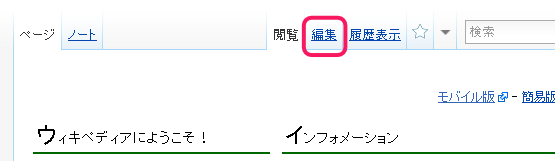
\includegraphics[width=10cm]{sample1.png}
\caption{図の挿入例}\label{サンプル図}
\end{figure}

これから常に使ってほしい大切な機能が「プレビューを表示」ボタンです.サンドボックスでなにか編集をして,それから「以上の記述を完全に理解し同意した上で投稿する」ボタンではなく,「プレビューを表示」ボタンを押してみましょう.そうすると,あなたがページに加えた変更の結果を,実際に保存する前に確認することができます.間違いは誰にでもあります.この機能は,間違いがないか自分で確認するためのものです.また,「プレビューを表示」ボタンを使えば,試しにページの体裁や表現をいろいろと変えてみても,ページの変更の記録にいちいち記録されずにすみますし,他にもいろいろと利点があるのです.でも,プレビューをした後,最後には保存するのを忘れないでください.

%図の挿入
\begin{figure}[htb]
\centering
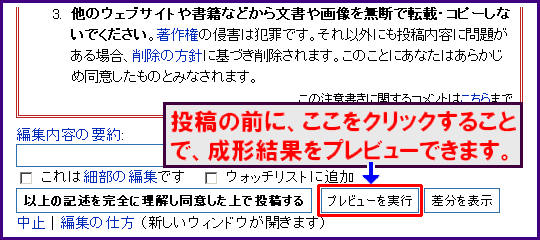
\includegraphics[width=10cm]{sample2.png}
\caption{図の挿入例}\label{サンプル図}
\end{figure}

「以上の記述を完全に理解し同意した上で投稿する」ボタンを押す前に、あなたが行った編集の説明を、編集用のテキストボックスと保存ボタンの間にある要約欄に書き込むようにしましょう。ウィキペディアでは、ここに編集の説明を書き込むことが大切なエチケットと考えられています。ただ単に誤字を直したような時には「誤字修正」と書けば充分です。文章の意味に影響を及ぼさないような、小さな修正のときには、要約欄の下にある「これは細部の編集です(説明)」のチェックボックスにチェックをいれておいてください(この機能はログイン時にのみ有効です)。

%図の挿入
\begin{figure}[htb]
\centering
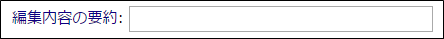
\includegraphics[width=10cm]{sample3.png}
\caption{図の挿入例}\label{サンプル図}
\end{figure}

Wikipediaの編集履歴データ

データCreative Commons Attribution-ShareAlike 3.0 Unported License (CC-BY-SA) および GNU Free Documentation License (GFDL) の下にライセンスされており (Wikipedia:著作権および利用規約を参照),再配布や再利用のためにデータベース・データの提供が行われています.データの生成は不定期に行われている.

Wikipediaではクロール行為のデータダウンロードは禁止されている.強引なクローリングは,Wikipediaが劇的に遅くなる原因となってしますためである.データベースから自動的にデータ収集している行為が発券された場合、システムの管理者から自身のサイトからWikipediaのアクセスを禁止されてしまう措置が起こってしまうこともある.また,ウィキペディア財団が法的措置を検討する場合もあるので,注意が必要.

%図の挿入
\begin{figure}[htb]
\centering
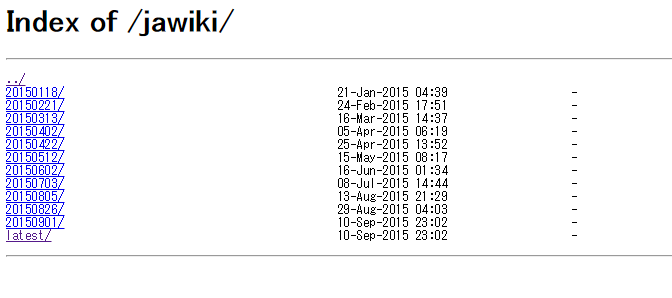
\includegraphics[width=10cm]{sample4.png}
\caption{図の挿入例}\label{サンプル図}
\end{figure}

ここに日本語版Wikipediaの履歴データが記録されている.

URLはhttps://dumps.wikimedia.org/jawiki/

他の言語もこのような形式で履歴データが残されている.他の言語のデータを取得したい場合はURLのhttps://dumps.wikimedia.org/○○wiki/の○○の部分を変更すればよい.言語は英語のスペルで頭文字2文字でよい.

例:英語の場合はスペルはEnglishなので,https://dumps.wikimedia.org/enwiki/とすればよい.



%図の挿入
\begin{figure}[htb]
\centering
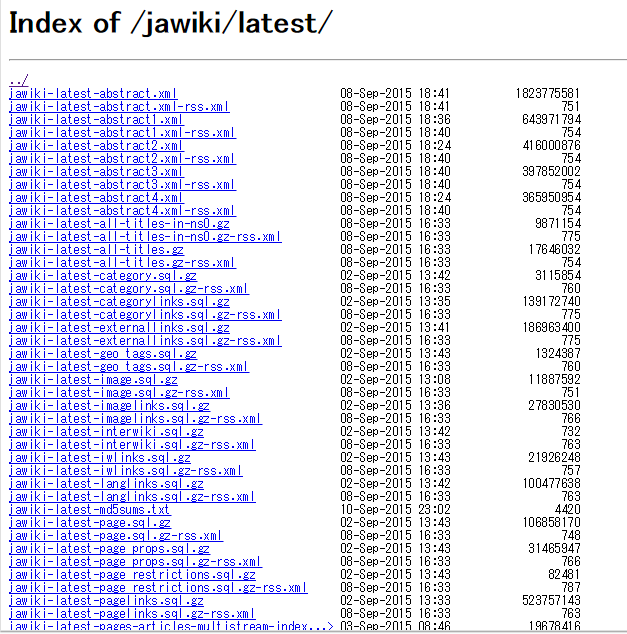
\includegraphics[width=10cm]{sample5.png}
\caption{図の挿入例}\label{サンプル図}
\end{figure}

どれか開くと上記のような画面になる.

ウィキページのデータはSQLのテーブルではなく、XMLで提供されている。XMLファイルの文字エンコーディングはUTF-8である。 非常にファイルサイズが大きいため、通常のエディタやブラウザで、解凍してはいけない。

データの詳細は下記のとおり

\begin{itemize}
 \item pages-articles.xml.bz2 - ノートページ、利用者ページを除く最新版のダンプ
 \item pages-meta-current.xml.bz2 - 全ページの最新版のダンプ
 \item pages-meta-history.xml.7z - 全ページの全ての版のダンプ
 \item all-titles-in-ns0.gz - 全項目のページ名一覧 (標準名前空間)
\end{itemize}

Wikipedia:編集回数の多いページの一覧

期間: 2014-07-01 — 2014-07-31 のランキング.

%図の挿入
\begin{figure}[htb]
\centering
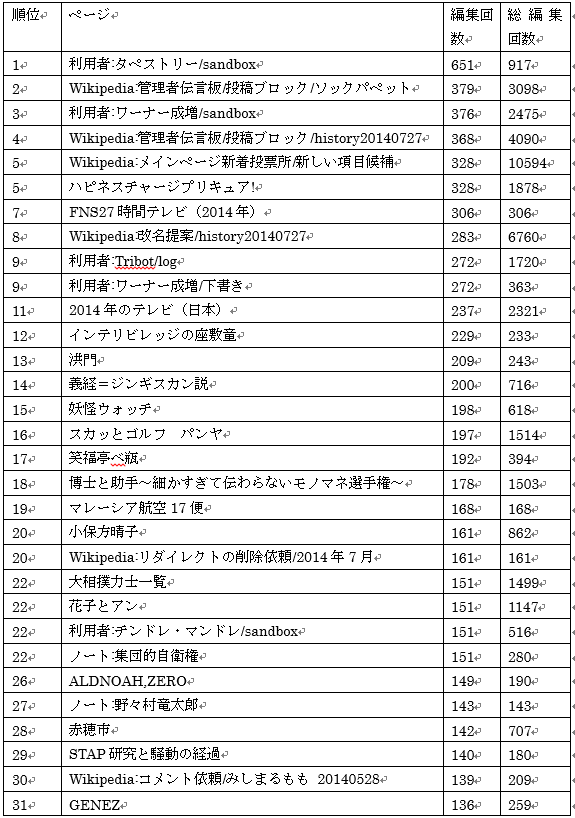
\includegraphics[width=13cm]{sample6.png}
\caption{図の挿入例}\label{サンプル図}
\end{figure}

%図の挿入
\begin{figure}[htb]
\centering
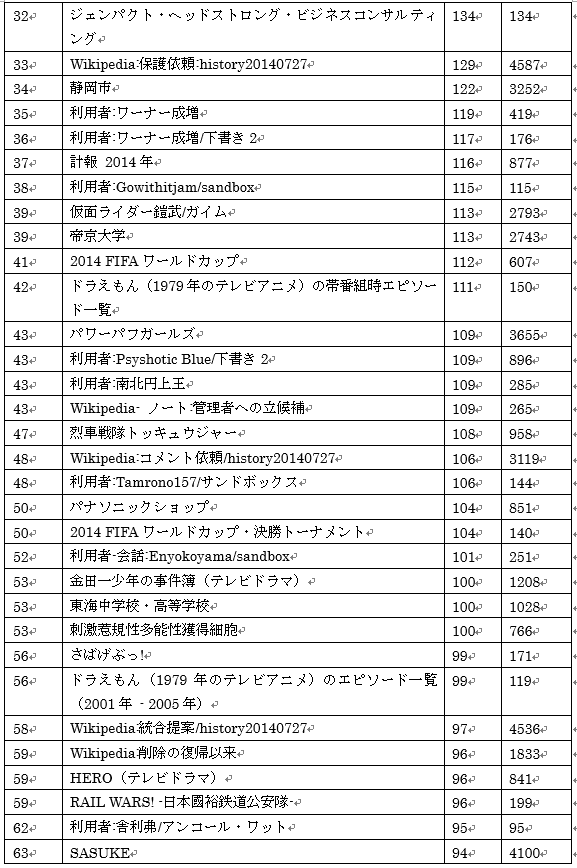
\includegraphics[width=13cm]{sample7.png}
\caption{図の挿入例}\label{サンプル図}
\end{figure}

%図の挿入
\begin{figure}[htb]
\centering
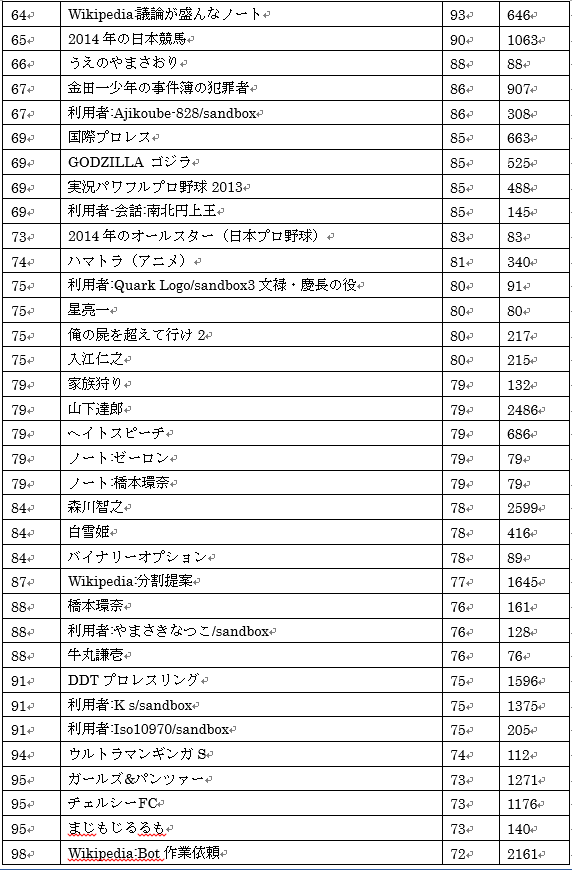
\includegraphics[width=13cm]{sample8.png}
\caption{図の挿入例}\label{サンプル図}
\end{figure}






\chapter{目的}

\chapter{手法}

\chapter{結果}

\chapter{考察}

\chapter{結論}

%図の挿入
\begin{figure}[htb]
\centering
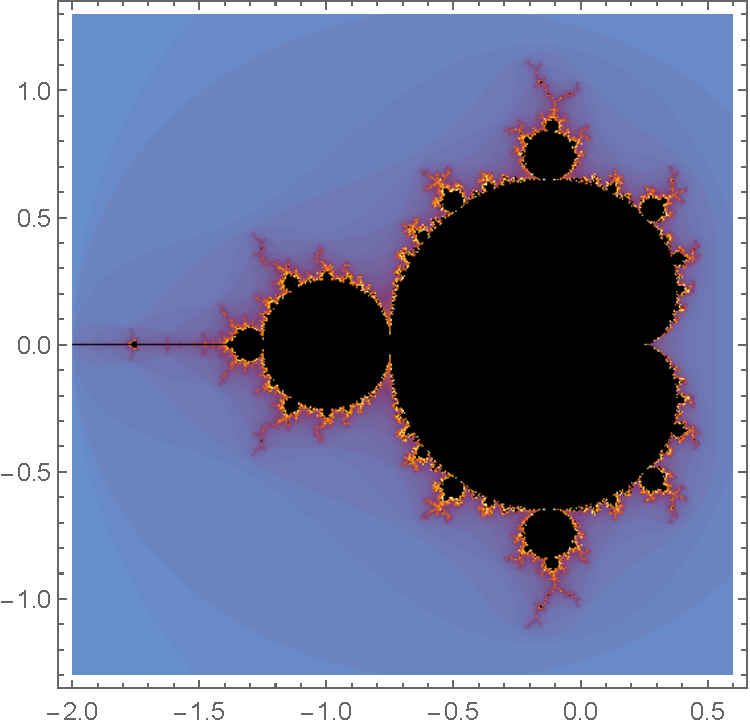
\includegraphics[width=10cm]{figure.pdf}
\caption{図の挿入例}\label{サンプル図}
\end{figure}

参考文献は文献ファイル(この文書では\verb|biblio.bib|)に記述し,\verb|\cite|で参照する.例:データベースのための問い合わせ言語SQLで数独を解く方法が提案されている\cite{yabuki2011}.このように参照すると,参考文献リストに自動的に登録される.文献の種類には,雑誌論文\cite{yabuki2011}や会議録論文\cite{yabuki2013},卒業論文\cite{kubo2014},書籍\cite{okumura2013},ウェブサイト\cite{self}などがある.文献の種類によって必要な項目が異なるため,\verb|biblio.bib|を見て確認すること.

\bibliographystyle{junsrt}
\bibliography{biblio}%「biblio.bib」というファイルが必要.

\end{document}